\subsection{Passungen}
    \begin{minipage}{0.99\linewidth}
        \begin{minipage}{0.49\linewidth}
            \begin{center}
                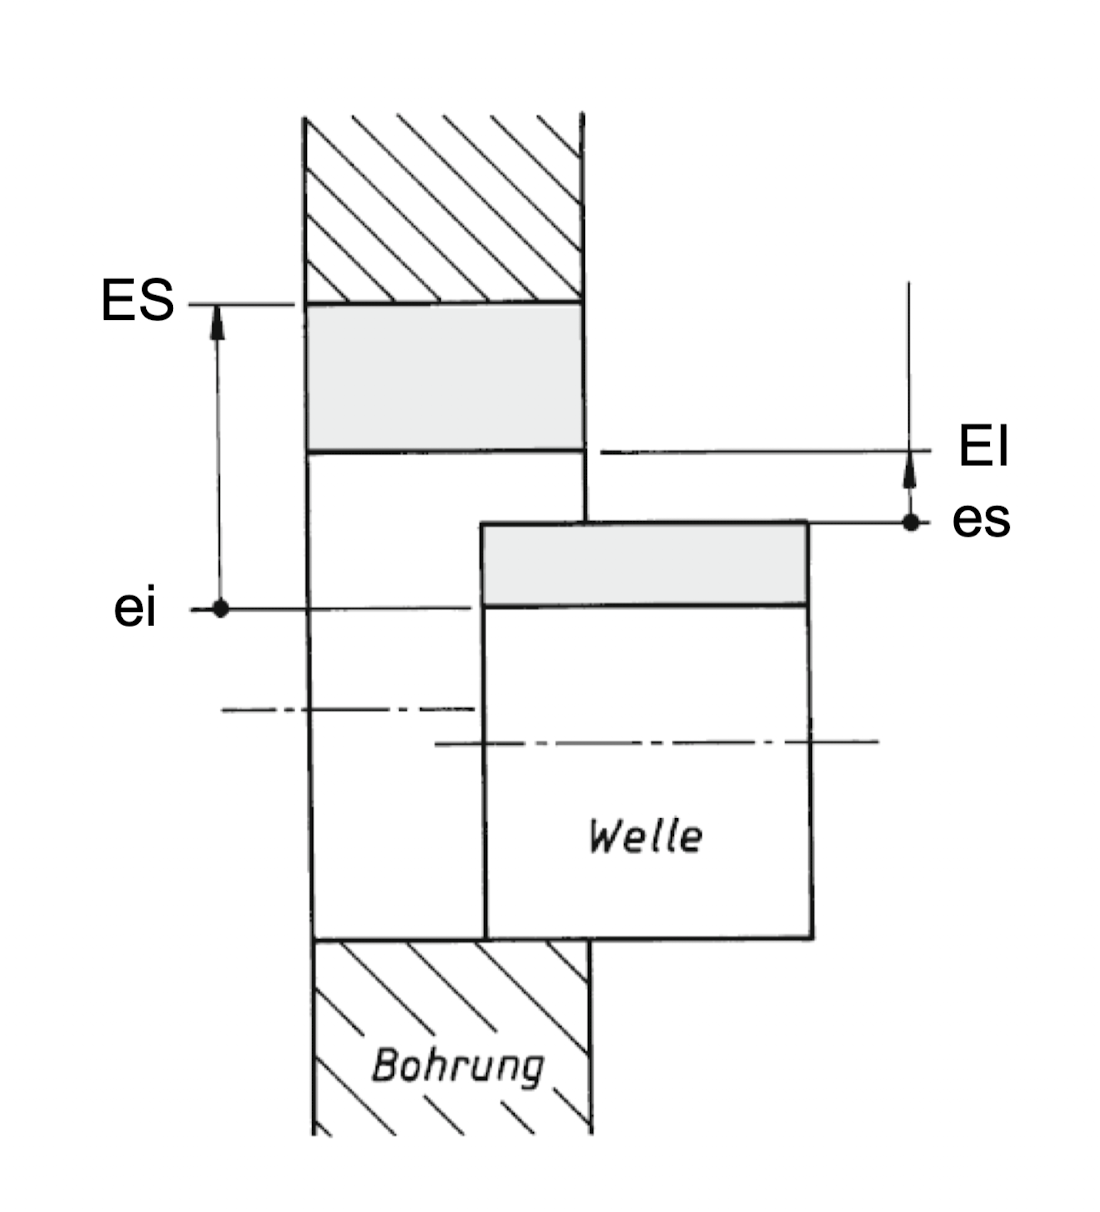
\includegraphics[width = 0.6\linewidth]{src/images/MAEIP_Spielpassung.png}
            \end{center}
        \end{minipage}
        \begin{minipage}{0.49\linewidth}
            Spielpassung
            \begin{align*}
                S_{min} &= EI - es\\
                S_{max} &= ES - ei
            \end{align*}
        \end{minipage}
    \end{minipage}
    \begin{minipage}{0.99\linewidth}
        \begin{minipage}{0.49\linewidth}
            \begin{center}
                \includegraphics[width = 0.6\linewidth]{src/images/MAEIP_Übergangspassung.png}
            \end{center}
        \end{minipage}
        \begin{minipage}{0.49\linewidth}
            Übergangspassung
        \end{minipage}
    \end{minipage}
    \begin{minipage}{0.99\linewidth}
        \begin{minipage}{0.49\linewidth}
            \begin{center}
                \includegraphics[width = 0.6\linewidth]{src/images/MAEIP_Übermasspassung.png}
            \end{center}
        \end{minipage}
        \begin{minipage}{0.49\linewidth}
            Übermasspassung

            \begin{align*}
                U_{min} &= ei - ES\\
                U_{max} &= es - EI
            \end{align*}
        \end{minipage}
    \end{minipage}